\documentclass[11pt]{article}
\usepackage{enumitem}
\usepackage{latexsym}

\usepackage{graphicx}
\usepackage{amsfonts}
\usepackage{amsmath,amssymb,amsthm}
\usepackage{xcolor}

\usepackage{tikz}
\usetikzlibrary{arrows}
\usetikzlibrary{automata}

\setlength{\textheight}{8.5in}
\setlength{\textwidth}{6.0in}
\setlength{\headheight}{0in}
\addtolength{\topmargin}{-.5in}
\addtolength{\oddsidemargin}{-.5in}

\input{preamble.tex}

\newcommand{\solution}[1]{\paragraph{Solution}  }

\begin{document}
\hw{3: Context-Free languages}{02/10/2026}{}{Due:03/03/2026}

This assignment is due on \textbf{11:59 PM, Thursday, March 3rd, 2026}. You may turn it in up to 48 hours late, but assignments turned in by the deadline receive 3\% extra credit.

You should submit a typeset or \emph{neatly} written pdf on Canvas.  The grading TA should not have to struggle to read what you've written; if your handwriting is hard to decipher, you will be asked to typeset your future assignments.

You may collaborate with other students, but any written work should be your own. 

\begin{enumerate}
    
\item \textbf{Short answer} (4 points)
\begin{enumerate}

\item (1 point - Both)
\\ Consider the CFG: \\ \\
$S \rightarrow AS | a$ \\
$A \rightarrow SA | b$ \\ \\
(i) Write out the derivation for $abba$ and draw the parse tree for the string $babbba$.
\begin{answer}
 For $abba$ the derivation would be as follows,
  \[
   S \to AS \to SA S \to SA AS \to aAAS \to abAS \to abbS \to abba
  \]

  For $babbba$ we have the tree as follows,
  \begin{center}
    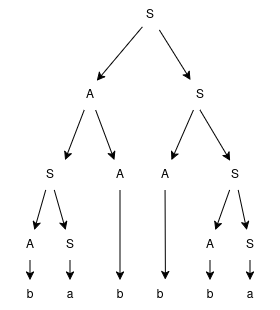
\includegraphics[width=.5 \linewidth]{img2}
  \end{center}
\end{answer}

\\ (ii) For a context-free grammar $G$ in Chomsky Normal Form, how many steps does a derivation of a string of $n$ letters have? (Answer should be an expression in terms of $n$ like $17n + 9,2003n^2$, etc.) Explain why.

\begin{answer}
  In Chomsky normal form each production can either point to a pair of non-terminals or a single terminal. Now given a string of length $n$ say with some arbitrary number of  steps / productions, to get a string with length $n + 1$, one of the terminals must be a non-terminal that branches out to generate 2 terminals. Note that we're removing 1 step (step to terminal) adding a step (step to 2 non-terminals) and adding 2 steps (a step each to a terminal for each of those 2 non-terminals).  Mathematically this can be seen as, 
  \[
    P(n) = P(n - 1) + 2
  \]

  Now for a string of length $1$, clearly we just have one step i.e one production. So we have, $P(1) = 1, P(2) = P(1) + 2 = 3, \dots$. So for an arbitrary $n$ we can solve this recursion by expanding it as follows, 
  \begin{align*}
    P(n) &= P(n - 1) + 2 \\
    &=P(n - 2) + 2 + 2 \\
    &= \dots \\
    &= P(1) + (n - 1)  \cdot 2\\
    &= 1 + 2n - 2 = 2n - 1
  \end{align*}

  So for a given string of length $n$ the total steps are $2n - 1$
\end{answer}

\item (1 point - Both) Let us define a context-free grammar $G$ to be in ``2-Form" if, for every nonterminal $A$, there are at most two options for replacing $A$ in a derivation. That is, there are at most two rules in $G$ that have $A$ on the left hand side, where the ``rule" $A \rightarrow B | C | D$ is considered to be three rules. Show that, for any context-free grammar, there is a 2-Form context-free grammar that recognizes the same language. 

\begin{answer}
  First consider our grammar $G$. Now let $A$ be an arbitrary non-terminal in this grammar that have more than two rules in $G$. So say we have $A \to X_{1} \mid X_{2} \mid \dots \mid X_n$, note here $A$ is an arbitrary non-terminal that has $n$ options. Now simply define a new non-terminal $A_{2} \to X_{2} \mid \dots \mid X_n$. So we have, $A \to X_{1} \mid A_{2}$ and $A_{2} \to X_{2} \mid \dots \mid X_n$, now $A_{2}$ is a non-terminal with $n - 1$ productions. So essentially we showed that for any arbitrary non-terminal $A$ with $n$ options we can write it as a pair of productions such that the maximum options are $n - 1$. Inductively we can continue doing this $n - 2$ times so that we end up with $n - (n - 2) = 2$ maximum productions. Hence we have a set of productions for $A$ such that the maximum options for each production is at most $2$. We can do this reduction for any arbitrary $A$ and $n$ in our grammar and hence we get a new grammer that accepts the same language but is 2-Form.
\end{answer}
    
\item (2 points - Section B) Let $G$ be a context-free grammar for a language $L$, and suppose $L$ contains only strings of length 2 or greater. Prove that there is a context-free grammar $G'$ which generates $L$ such that every rule of $G'$ has the form $A -> x_1x_2$, where $A$ is a nonterminal, and each $x_i$ is a terminal or nonterminal.

\begin{answer}
    % Enter your solution here!

\end{answer}
    
\item (2 points - Section X) Consider a context-free grammar in Chomsky normal form which has $n$ variables. Prove that if there is some string $s \in L(G)$ such that the derivation of $s$ has atleast $2^{n}$ steps, then $L(G)$ is infinite. (Hint: Think about the parse tree for $s$)


\begin{answer}
  In Chomsky normal form each variable / non-terminal goes to either two non-terminals or a terminal. Now consider the binary parse tree. Now in the parse tree at each level the number of leaves is at most $2^{h}$ (and $2^{h}$ for a perfect tree) where $h$ is the level / height. Now we know from (a) that if we have a length $k$ string then we must have $2k - 1$ steps. So if our string $s$ has at least $2^{n}$ steps, this means we have $2k - 1 \ge 2^{n}$ which gives us $k \ge 2^{n - 1} + 1 / 2$ which means $k \ge 2^{n - 1} + 1$ as $k$ must be an integer. This means the length of our string is greater than equal to $2^{n - 1} + 1$. Now note that the smallest height tree we can have given a fixed number of leaves is a complete tree. Now in a perfect tree of height $h$ we have $2^{h}$ now the minimum height we can have is $h$ so that $2^{h} \ge 2^{n - 1} + 1$. Now note that the power of $2$ that is greater than $2^{n - 1}$ is only $2^{n}$. So we have $h \ge n$. Where $n$ is the number of variables. Note that $h$ starts from $0$, so at a height of $n$ there exists $n + 1$ nodes, but now note that if we have $n + 1$ nodes for at least one path in our tree but only $n$ variables, this means that there is a repetition. In other words there is some $X$  such that $X \to^{+} X$ i.e some path to get from $X$ to itself. But if there is such a path then this means that we can go down this path an infinite number of times as we can repeat $X$ to itself infinite number of times, each time we repeat it corresponds to a new string in our language. This means our language is infinite.
\end{answer}
    
\end{enumerate}

    
\item \textbf{Context Free Grammars} (4 points)

Give context free grammars for the following languages:
\begin {itemize}
\item (Section B) $L_1 = \{a^ib^jc^kd^l\ |$ $i=j$ or $k=l$ but not both, $i,j,k,l \geq 0\}$

\begin{answer}
    % Enter your solution here!

\end{answer}

\item (Both) $L_2 = \{1^i0^j\ |$ for some nonnegative $x,y \in \mathbb{Z}, $ $x+y = i$ and $5x+2y = j\}$

\begin{answer}
  To solve this we can note two things. Every time $i$ is incremented by 1, either $x$ is incremented by 1 or $y$ is. But if $x$ is incremented by $1$ then $j$ will by $5$ as $y = 5x + 2y$ and similarly if $y$ is incremented by $1$ then $j$ will be incremented by $2$. So all in all we have two choices to take. The grammar would look like,
  \begin{align*}
    S &\to AB\\
    A & \to 1^{1} A 0^{5} \mid \epsilon\\
    B &\to 1^{1} B 0^{2} \mid \epsilon
  \end{align*}
\end{answer}
    
\item (Section X) $L_3 =$ the \textit{complement} of $\{ww\ |\ w \in \Sigma^*\}$. 

\begin{answer}
  Consider for simplicity we have $\Sigma = \{a, b\}$, now we will generate a CFC for $L_{3}$. First we generate all odd length strings centered on $a$ and $b$. Trivially, this is in $L_{3}$ because we can't write it as $ww$ where $w \in \Sigma^*$. So consider the following CFG, 
  
  \begin{align*}
    S &\to A \mid B\\
    A &\to aAa \mid aAb \mid bAb \mid bAa \mid a\\
    B &\to aBa \mid aBb \mid bBb \mid bBa \mid b
  \end{align*}

  Note that this grammar gives us all odd length strings. $A$ allows for any combination of strings on the outside and the only non-terminal is $a$ which will have to end up in the center, similar for $B$.

  \vspace{1em}
  
  Now we have to generate even length strings that are not the concatenation of two equal strings. So consider the strings $AB$ and $BA$ clearly as $A$ and $B$ are odd length their concat are even length. So our new grammar is, 
  
  \begin{align*}
    S &\to A \mid B \mid AB \mid BA\\
    A &\to aAa \mid aAb \mid bAb \mid bAa \mid a\\
    B &\to aBa \mid aBb \mid bBb \mid bBa \mid b
  \end{align*}
  But we still need to show that their concatenation could never be split into two strings that are equal. So WLOG consider $AB$ where $|A| = 2m + 1$ and $|B| = 2n + 1$ and $m < n$. Now what we need to ensure is that the centers of $A$ and centers of $B$ are NON-equal as we know A  and B are centered by $a$ and $b$ respectively. So in $AB$ the center of $A$ i.e $a$ is at position $m + 1$ and for $B$ is $n + 1$. Now the absolute center of the string $AB$ is at $(2m + 1 + 2n + 1) / 2 = m + n + 1$. Now consider our string is $w v$ where $|w| = |v|$ then $v$ starts at position $m + n + 2$. Now relative to $w$ the center of $A$ is at position $m + 1$. And relative to $v$ the center of $B$ would be at the absolute position of the center - middle of the string. The absolute position of the center of $B$ is at $2m + 1 + (n + 1)$ and the middle as we know is $m + n + 1$ so our relative position is $2m  + 1 + n + 1 - m - n - 1 = m + 1$. Note now that at position $m + 1$ for string $w$ we have the center of $A$ which is $a$ and at position $m + 1$ of string $v$ we have the center of $B$ which is $b$. But clearly as $|w| = |v|$ this means that the string $w$ can never be equal to $v$ as we just showed that the position $m + 1$ will always be unequal. This means we can never have $ww$ as a part of our language.
\end{answer}
    
\end{itemize}



\item \textbf{Pushdown Automata} \textit{**Both Sections**}(4 points)

Give pushdown automata for the following languages. You may assume $\Sigma = \{0, 1\}$.
\begin{itemize}
    \item $L_4 = \{w0w^{\mathbb{R}}\ |\ w \in \Sigma^*\}$, the set of palindromes with a $0$ as the middle character

    \begin{answer}
      Our PDA is as follows,
      \begin{center}
        \begin{tikzpicture}[shorten >=1pt,node distance=2cm,on grid,auto,scale=0.17]
\tikzset{accepting/.style={double distance=1mm}}
\node[state,initial, label=center:{$q_0$}] (0) at (15.5,-26) {};
\node[state, label=center:{$q_1$}] (1) at (30.2,-25.8) {};
\node[state, label=center:{$q_2$}] (2) at (44.6,-25.8) {};
\node[state,accepting, label=center:{$q_3$}] (3) at (59.1,-25.8) {};
\path[->] (0) edge node [swap] {$\varepsilon,~\varepsilon~\rightarrow\$$} (1);
\path[->] (1) edge[loop above] node {$0, \epsilon \rightarrow 0$} ();
\path[->] (1) edge[loop below] node {$1, \epsilon \rightarrow1$} ();
\path[->] (1) edge node [swap] {$0,~\varepsilon~\rightarrow\varepsilon$} (2);
\path[->] (2) edge[loop above] node {$0, 0 \rightarrow \epsilon$} ();
\path[->] (2) edge[loop below] node {$1, 1 \rightarrow \epsilon$} ();
\path[->] (2) edge node [swap] {$\varepsilon,~\$~\rightarrow\varepsilon$} (3);
\end{tikzpicture}
      \end{center}

      Note that first from $q_{0} \to q_{1}$ we have an $\epsilon$ transition where we append $\$$ to the stack that will represent the bottom of the stack. Now we will start consuming $w$. Note that at $q_{1}$ we have two high level choices, one is to consume $w$ and one is to guess the middle $0$ and leave. So for consuming $w$ for any alphabet $a \in \{0, 1\}$ we push $a$ onto the stack when we encounter it. Now when we encounter the middle $0$ we don't push or pop the stack and just move to the state $q_{2}$ which represents the reverse string. At $q_{2}$ now note that both our non-epsilon transitions are dependent on the stack top. So if we get a $1$ and a $1$ is at the top then we pop and we do the same for for a $0$. This ensures that the sequence of letters we get are the reverse of what was pushed to the stack. Clearly if we have either $1, 0$ or $0, 1$ we have no where to go and naturally we don't accept the string. Now if we ever pop every alphabet from $\Sigma$ off the stack we will be left with $\$$ for which we have an $\epsilon$ transition that will go to $q_{3}$ the accepting state.

      
    \end{answer}
        
    \item $L_5 = \{w\ |\ w\text{ is odd length but is not a palindrome}\}$ 

    \begin{answer}

      We have two conditions, first $w$ is odd length and second $w$ is not a palindrome. Now if $w$ is odd length then it means we can split $w$ as $axb$ where $|a| = |b|$ and $x \in \Sigma$. So we can ensure it's odd length by guessing $x$ in our PDA and moving to another state where we implicitly count $b$. Secondly, to ensure it's not a palindrome we $a$ to our stack guess $x$ and start popping $b$ from the stack, if it ever doesn't match then we move to a state where we just count the rest of the letters and if it's equal in length we just accept, if it matches all the way to the bottom then we know that it's a palindrome and hence we reject. The PDA looks like,

      \begin{center}
        \begin{tikzpicture}[shorten >=1pt,node distance=2cm,on grid,auto,scale=0.17]
\tikzset{accepting/.style={double distance=1mm}}
\node[state,initial, label=center:{$q_0$}] (0) at (12.8,-25.8) {};
\node[state, label=center:{$q_1$}] (1) at (25.1,-25.8) {};
\node[state, label=center:{$q_2$}] (2) at (41.2,-25.8) {};
\node[state, label=center:{$q_3$}] (3) at (73.2,-36) {};
\node[state, label=center:{$q_4$}] (14) at (61.7,-11.8) {};
\node[state,accepting, label=center:{$q_5$}] (15) at (73.2,-11.8) {};
\path[->] (0) edge node [swap] {$\varepsilon,~\varepsilon~\rightarrow\$$} (1);
\path[->] (1) edge[loop above] node {$0, \epsilon \rightarrow0$} ();
\path[->] (1) edge[loop below] node {$1, \epsilon \rightarrow1$} ();
\path[->] (1) edge[bend right=25 , swap] node {$0,~\varepsilon~\rightarrow\varepsilon$} (2);
\path[->] (2) edge[loop above] node {$0, 0 \rightarrow \epsilon$} ();
\path[->] (2) edge[loop below] node {$1, 1 \rightarrow \epsilon$} ();
\path[->] (2) edge node [swap] {$\varepsilon,~\$~\rightarrow\varepsilon$} (3);
\path[->] (1) edge[bend left=25 ] node {$1,~\varepsilon~\rightarrow~\varepsilon$} (2);
\path[->] (2) edge[bend left=25 ] node {$0,~1~\rightarrow~\varepsilon$} (14);
\path[->] (14) edge node [swap] {$ \epsilon, \$ \rightarrow \epsilon$} (15);
\path[->] (2) edge[bend right=25 , swap] node {$1,~0~\rightarrow~\varepsilon$} (14);
\path[->] (14) edge[loop above] node {$(0, 1), (0, 1) \rightarrow\epsilon$} ();
\end{tikzpicture}
      \end{center}
      
      So first we add a $\$$ to the stack to represent the bottom. Now for each string with $0$ and $1$ the state $q_{1}$ will add the symbol to the stack, then we will guess the center symbol, be it $0$ or $1$ without changing the stack and move to state $q_{2}$ which represents the second half after the middle. At $q_{2}$ we have three high level cases, first we match the alphabet in the top of the stack, in this case we just pop the stack and continue to stay in $q_{2}$, second if we don't match the top of the stack we move to state $q_4$ and third we reached the end of the stack. Now note if we reach the end of the stack the second half matched perfectly with the stack's pops which means the string is a palindrome and as $q_{3}$ is a sink state we reject automatically. Now, going back to the second case if we don't match then we know we can never have a palindrome but we still need to count whether we have the same number of symbols as in the stack (if we have the same it implies we guessed the middle right and that we have an odd length string), so at $q_{4}$ for any symbol $a \in (0, 1)$ for any top of the stack (if it's 0 or 1), we pop it (note that if we guess the middle wrong early, then we end up popping everything in the stack until the $\$$ at which point we don't have any transitions and hence reject). The point is we just want to count the symbols so it's enough to just pop the stack until we reach the bottom.



    \end{answer}
        
\end{itemize}

\item [4.] \textbf{Pumping Lemma} \textit{**Both Sections**}(4 points)

Show that $\{x_1\star x_2\star...\star x_t ~|~ t > 1, x_i \in \{a,b\}^*, \text{ and } \exists x_i,x_j \text{ with } i \neq j \text{ but } x_i = x_j \}$ is not context-free using the pumping lemma for context free languages.

\begin{answer}
  First we assume that it is context free and take the pumping length to be $p$, so we know that for any string $s \in L$ such that $|s| > p$ we have $s = uvxyz$ such that all $uv^{i}xy^{i}z \in L$ while $|vy| > 0$  and $|vxy| \le p$.
  \vspace{1em}
  
  Now choose our string $s = a^{p}b^{p} \star a^{p}b^{p}$. Now we need to consider all possible $|vxy|$ such that the length is smaller than $p$. So note for all substrings of length smaller than $p$ we have three choices (note these choices are exhaustive, i.e it covers all cases),
  \begin{enumerate}
    \item $vxy$ is a substring of $x_1$, so this means that it's a part of the first string.

      \qquad Now in this case if $vxy \subset x_{1}$, then note that for any choice of $vy$ such that $|vy| > 0$, if we pump $v$ and $y$ then we trivially increase (or decrease if $i = 0$) the size of the string $x_{1}$. However this means that we can never have $x_{1} = x_{2}$ because $|x_{1}| \ne |x_{2}|$.
    \item $vxy$ exists in the second half i.e a substring of $x_{2}$. 

      \qquad Similar to case (a) we have size of $x_{2}$ can be pumped to be greater than size of $x_{1}$ which wil trivially make it non-equal and out of our language.

    \item $vxy$ exists in the middle, so this means we have $\star$ a substring of $vxy$. Now 

      \qquad In this case note that our string is $a^{p}b^{p}\star ba \star a^{p}b^{p}$ and we know our string is length smaller than equal to $p$ and contains $\star$. So the only possible way is if we have $vxy = b^{i}\star a^{j}$ where $i + j < p$. Now note we have different possibilities for $v, x, y$ for this. Consider two cases that are exhaustive, (1) $v$ is entirely a substring of $b^{i}$ and let $x y$ be anything. Here if we pump $v$ note that we change the total number of $b$ in the string $x_i$ but $xv$ does NOT contain any $b$ so we can never change the number of b's in string $x_{2}$ no matter our choice of $y$. So this necessarily means $x_{1} \ne x_{2}$ for all choices of $x$ and $y$. (2) We have $v$ is entirely in the second half i.e $a^{j}$, we have have a similar problem as (1) as we can increase the number of $a'$ in $x_{2}$ while not being able to change anything of $x_{1}$ hence $x_{1} \ne x_{2}$. (3) Last case is when $v$ contains the $\star$, now in this case note that no matter the configuration of $v, x$  or $y$ if we choose $i = 0$ we necessarily have the $ \star $ disappear as we have $v^{0}$ and $v$ contains the only $\star$. But note that our language necessarily has $t > 1$  which means that a string $x_i \in \{a, b\}*$ is not accepted by the language.
  \end{enumerate}

  Hence, we just showed for any valid decomposition we have a contradiction.
\end{answer}

\end{enumerate}
\end{document}
